\documentclass[article]{BJTU-thesis}
\usepackage{url}
\usepackage{booktabs}
\usepackage{subcaption}
\setcounter{tocdepth}{4}
\setcounter{secnumdepth}{4}
\hypersetup{hidelinks}
\renewcommand\thesection{\arabic {section}}
\renewcommand\thefigure{\arabic {figure}}
%%%%%%%%%%%%%%%填写封面信息%%%%%%%%%%%%%%%%%%%%
%\authora{汤新宇  17301137}
%\authorb{陈嘉琪  17301060}
%\authorc{刘歆怡  17301129}
\authora{唐麒}
\authorb{17301138}
%\authorf{张钰铎  17301145}
%\comment{同{\color{white}哈}等{\color{white}哈}贡{\color{white}哈}献}
%\studentNumber{16121248}
\advisor{冀振燕}
%\advisorTitle{教授}
%\degreeType{学术型}
%\major{机械制造}
%\researchArea{切削力分析}
\title{结构光三维重建软件\\设计模式分析}
\bibliographystyle{unsrt} % BibTex
%\englishtitle{The Path Planning of Blade Machining Tool Based on Cutting Force Analysis.}
%%%%%%%%%%%%%%%%%%%%%%%%%%%%%%%%%%%%%%%%%%%%%%
%\setmainfont{Times New Roman}
\bibliographystyle{unsrt} % BibTex
\begin{document}
	\makecover
	
	\tableofcontents
	\newpage

	\newpage
	\setcounter{page}{1}
	\section{项目简介}
     近年来,为了适应社会发展的需求,铁路向着高速、重载、高密度运行方向发展,尤其是在高速铁路领域,我国已经成为世界运营里程最长,动车组开行最多的国家。
     
     高铁的轮轨姿态反映了车轮与钢轨之间复杂的动态相互作用和约束关系,掌握他们之间真实接触姿态是保障高速铁路安全运营的重要基础。但仅从二维图像上获取轮轨接触姿态是不精确、不可靠的,需要将轮轨表面的特征点提取出来,重建出一个三维模型,才能更加真实正确地获得轮轨接触姿态。但由于高铁轮轨表面相对光滑且无明显特征点,造成特征不易提取,使得重建精度较差。此外,高铁列车的快速运行速度快也给轮轨表面特征点的提取提出了严峻挑战。
  
 	 三维重建技术是计算机视觉技术的一个重要分支,是计算机视觉和计算机图像图形学相结合的一个热门研究方向。根据测量时是否与被测物体接触可分为接触式测量与非接触式测量。其中,编码结构光法是一种主动式的非接触式测量方法,具有成本低,精度高,易于实现等优点。
 	 
     \begin{figure}[!htbp]
     	\centering
     	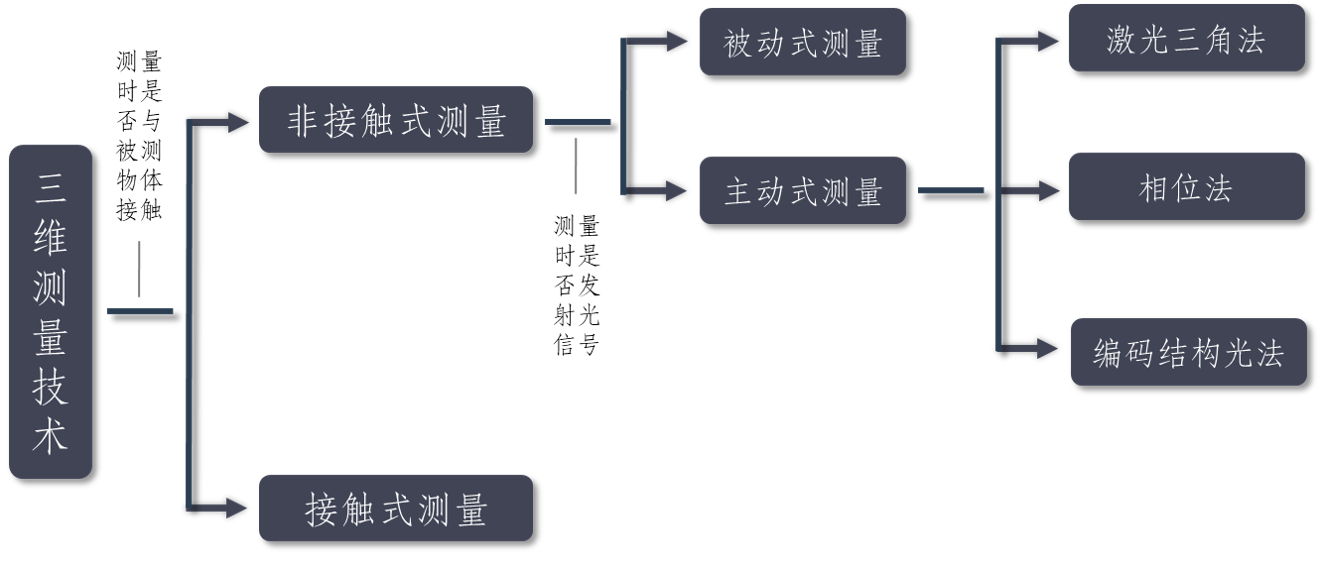
\includegraphics[scale=0.7]{0.png}
     	\caption{三维重建技术}
     \end{figure}
     
     编码结构光法利用投影仪投射出的一定模式的编码结构光图案对目标物体进行编码,利用摄像机获取物体图像,通过计算机对所得图像进行解码处理,利用摄像机中的图像点和投影仪中的点对应关系计算物体表面点的空间坐标,获得物体的三维信息,从而还原物体三维形状。
 
	 \begin{figure}[!htbp]
	 	\centering
	 	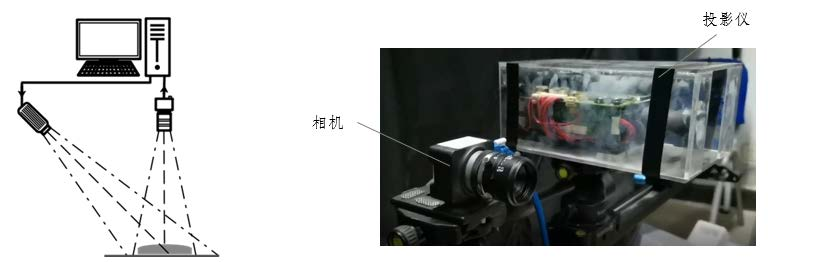
\includegraphics{1.png}
	 	\caption{结构光系统}
	 \end{figure}
 
     编码结构光法三维重建技术主要由系统标定、结构光编码、图像获取、结构光解码和三维坐标计算等5个关键技术组成。
 		\begin{itemize}
 			\item 系统标定:结构光系统标定包括摄像机和投影仪的标定,从而获取摄像机和投影仪的内外参数;
 			\item 结构光编码:通过编码的方式使图像每一点的“身份”可以被识别;
 			\item 结构光解码:通过一定的解码方案将摄像机采集的投射在目标物体上的结构光图案的二维畸变图像解码;
 			\item 三维坐标计算:结合标定好的系统参数,由光学三角测距原理获获得物体的三维信息。 									
		\end{itemize}
	
	结构光编码方案依据编码策略主要分为时间编码和空间编码两大类。\textbf{时间编码}结构光法是对目标物体表面投射一系列不同的编码图案,获得一组编码图像序列,标记目标物体上同一点在不同时间点的,经过处理获取这一点的结构光。\textbf{空间编码}结构光法能够通过向目标物体投射一幅编码图案,将获得的编码图像与投影图案对照进行解码,获取物体的三维信息。
	
     空间编码的特点是投影图案只有1幅,图案中每点的码字根据其周围邻近点的信息(如像素值、颜色或几何形状等)得到,适合与动态场景的三维重建。空间编码常用的编码方式主要有基于基于 $De \;Bruijn$ 序列的编码和基于 $M-$ 阵列 的编码。   
		
	综上所述,本项目以机器视觉理论和方法为基础,重点研究基于编码结构光的高铁轮轨姿态三维重建方法。通过编码结构光获取轮轨稠密三维点云数据,三维重建高铁轮轨姿态模型,并实现可视化。
	
     \section{项目展示}
    近年来,关于编码结构光法三维重建的研究层出不穷。但现有的基于空间编码结构光的重建方法普遍存在计算时间长、点云稠密度低等问题。为了解决现有方案存在的问题,结合本项目的实际运用场景,设计了基于 $De \;Bruijn$ 序列的条纹模式,同时在图像的 V 通道编码了相位信息。在解码的过程中,通过对拍摄获得的图像进行条纹中心点的分析和小波分析,将二者的分析结果相机和,即可提高点云的稠密度,并避免了相位展开引入的误差,在重建速度上也有一定的改善。 
     
     在此实验方案的基础上,设计并实现了结构光三维重建软件,根据结构光系统进行三维重建的需求,本软件可分为相机标定、三维重建和点云渲染三个模块,下面分别对三个模块的功能进行介绍。
     \begin{itemize}
     	\item 系统标定模块
     	\begin{figure}[!htbp]
     		\centering
     		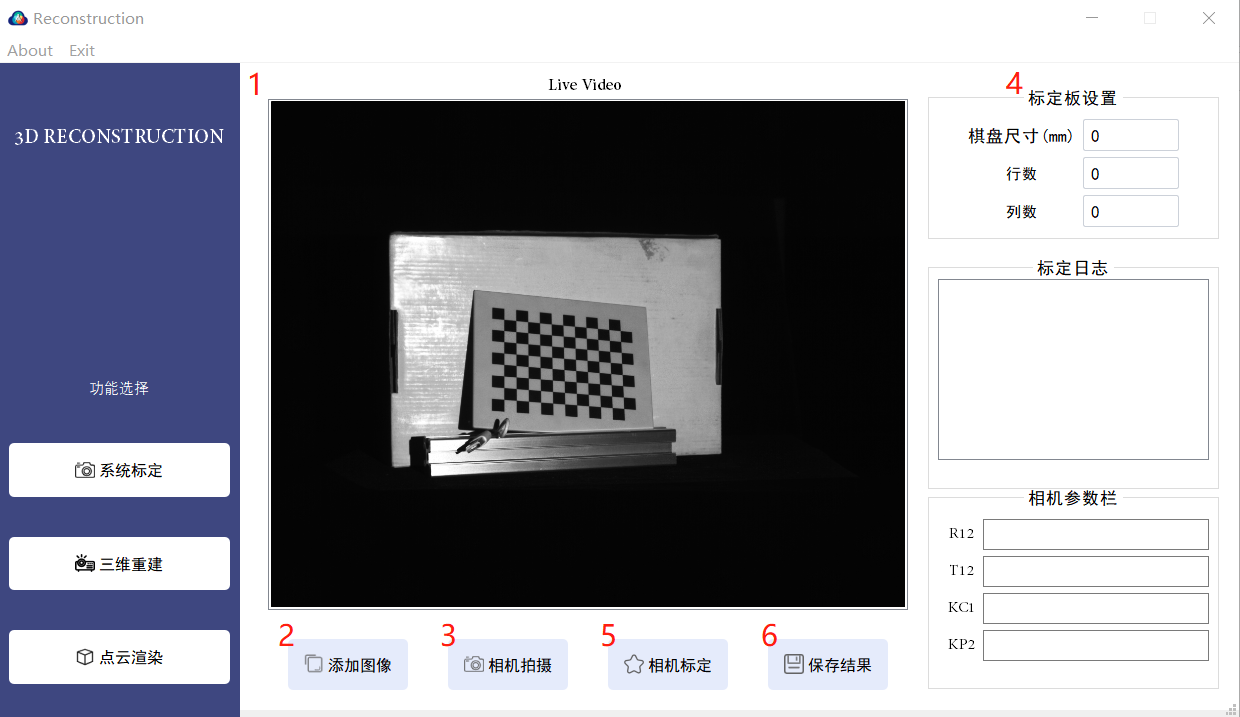
\includegraphics[scale=0.5]{2.png}
     		\caption{系统标定界面}
     	\end{figure}
     \begin{itemize}
     	\item[$\blacksquare$] 配置相机和投影仪
        \item[$\blacksquare$] 上传标定图像
     	\item[$\blacksquare$] 相机拍摄
     	\item[$\blacksquare$] 设置标定板参数
     	\item[$\blacksquare$] 相机(相机和投影仪)标定
     	\item[$\blacksquare$] 保存标定结果
     \end{itemize}
 \newpage
     \item 三维重建模块
     \begin{figure}[!htbp]
     	\centering
     	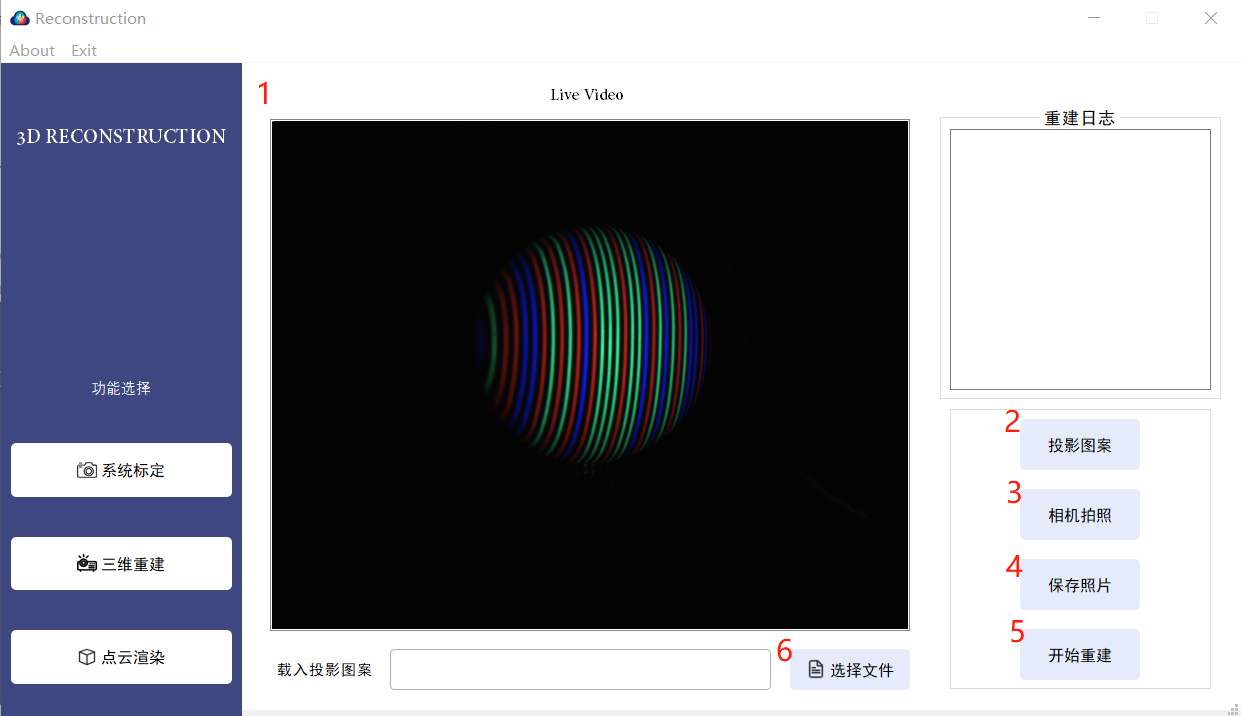
\includegraphics[scale=0.6]{3.png}
     	\caption{三维重建界面}
     	\label{fig:fig1}
     \end{figure}
 \begin{itemize}
 	\item[$\blacksquare$] 投影编码图案
 	\item[$\blacksquare$] 拍摄投影图像
 	\item[$\blacksquare$] 上传本地图像
 	\item[$\blacksquare$] 保存拍摄图像
 	\item[$\blacksquare$] 进行三维重建
 	
 \end{itemize}
 \item 点云渲染模块
 \begin{figure}[!htbp]
 	\centering
 	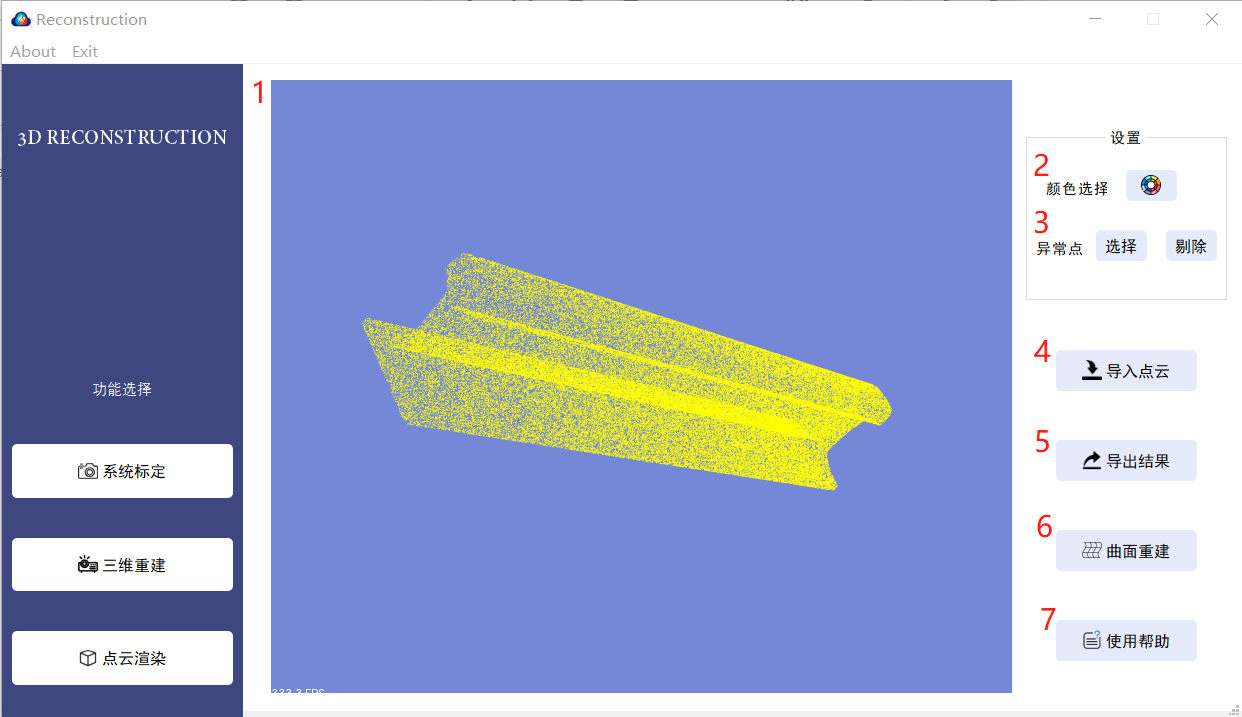
\includegraphics[scale=0.6]{4.png}
 	\caption{点云渲染界面}
 \end{figure}

\begin{itemize}
	\item[$\blacksquare$] 渲染点云
	\item[$\blacksquare$] 改变点云颜色
	\item[$\blacksquare$] 异常点选择和剔除
	\item[$\blacksquare$] 泊松曲面重建
	\item[$\blacksquare$] 导出点云数据
	\item[$\blacksquare$] 使用帮助
	
\end{itemize}
     \end{itemize}
		
\section{设计模式的运用}
在软件工程中,设计模式指的是解决软件设计中常见问题的一种通用的,可重用的解决方案,用于详细设计阶段,是为了解决局部的设计问题。设计模式不是一种可以直接转换成代码的集成设计,关注于某一特定的面向对象设计领域的问题,是一种图和解决问题的描述或模板。

在本项目中运用了例如单例模式的创建型设计模式\footnote{创建型模式是创建对象,而不是直接实例化对象的模式,可以灵活确定特定情况下创建什么对象。}和代理模式的结构性模式\footnote{结构型模式是将一组对象组合为一个更大的结构体的模式,描述类与对象如何结合组成更大的结构。},在经过分析之后,项目的部分功能实现还可以采用包含责任链模式(一种行为型模式\footnote{行为型模式一种定义系统中对象之间的通信、以及复杂程序中流的控制的模式,行为型模式关心对象之间的通信、流的控制。})在内的其他设计模式,下面对不同的设计模式及其在本项目中的应用进行详细介绍。
\subsection{单例模式}
	
单例模式是一种创建型模式,他是为了保证一个类只有一个对应的实例被创建,并提供一个指向这一单一实例的全局指针。单例模式的参与者是参与此种模式的类或对象。其类图如下图所示:

	 	\begin{figure}[!htbp]
		\centering
		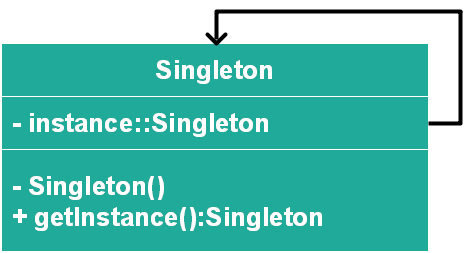
\includegraphics[scale=1]{5.png}
		\caption{单例模式类图}
	\end{figure}

\newpage

参与单例模式的类定义了让用户访问其唯一实例的实例化操作和获取实例方法的操作,其中获取实例方法是一个类操作。此外,这个类还负责创造和维护唯一实例。

单例模式有三种实现方式,
	 	\begin{figure}[!htbp]
	\centering
	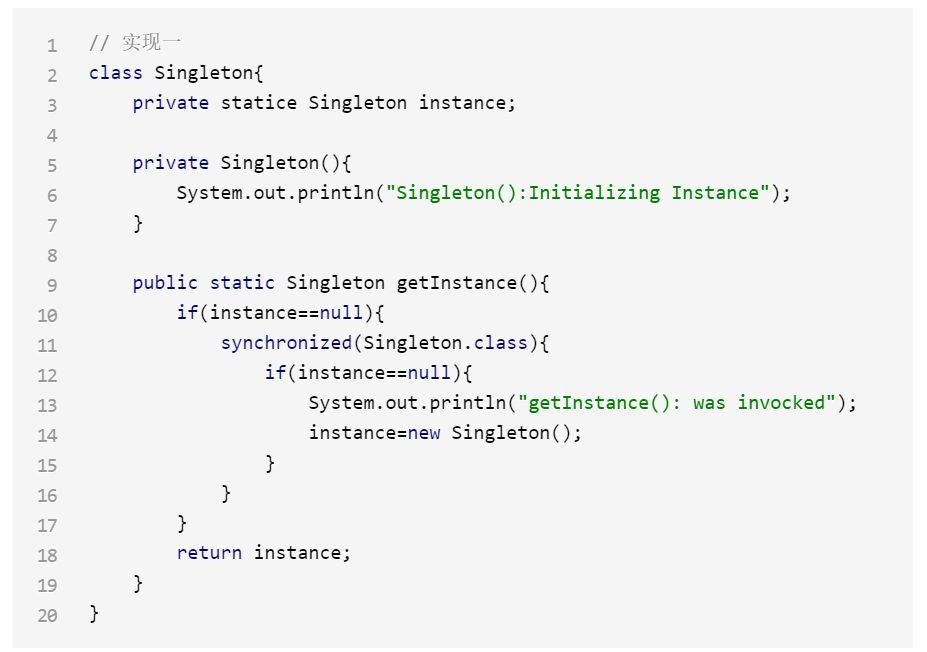
\includegraphics[scale=0.5]{6.png}
	\caption{单例模式实现方法——双重检验锁}
\end{figure}

	 	\begin{figure}[!htbp]
	\centering
	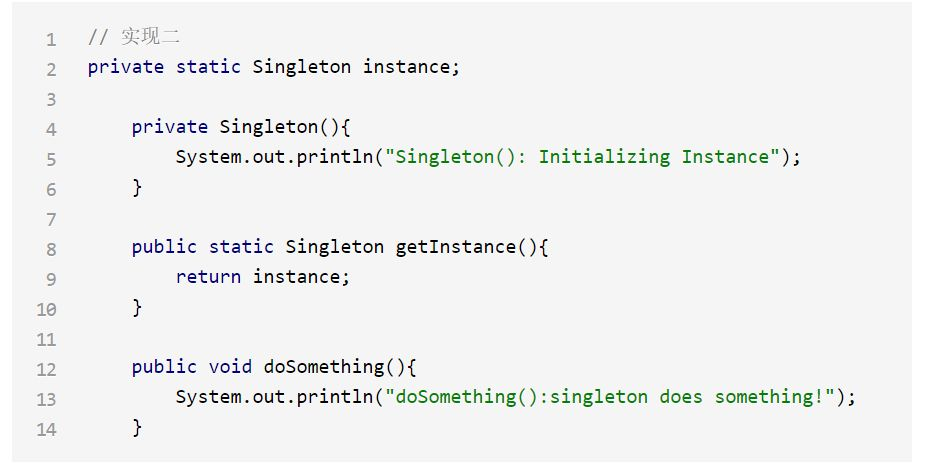
\includegraphics[scale=0.5]{7.png}
	\caption{单例模式实现方法——懒汉式,线程不安全}
\end{figure}


	 	\begin{figure}[!htbp]
	\centering
	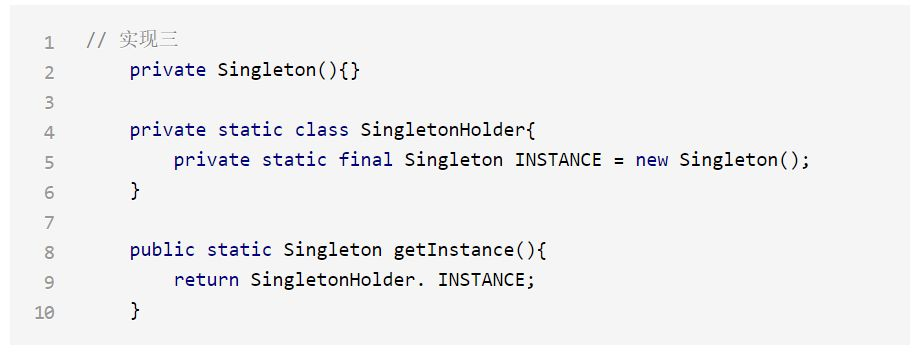
\includegraphics[scale=0.5]{8.png}
	\caption{单例模式实现方法-静态内部类}
\end{figure}

	需要注意的是第而中实现方法在多线程的情形下,有可能会创建多个实例。
	
	在本项目中有多处使用单例模式,如类 $Camera$ 和 $Projector$,分别用来初始化、控制相机和投影仪完成标定、拍摄等功能。
	
	正如在上一节所介绍的,本系统由相机、投影仪和计算机三部分组成,软件的部分功能依赖于相机和投影仪,因此需要通过驱动、接口等获得相机、投影仪的实例,从而可以控制相机和投影仪进行拍摄等。
	
	在系统标定模块,投影仪需要在标定板上投影一组图片,相机保持与投影相同的帧率进行拍摄,通过拍摄获得的图片,软件可以进行系统标定,从而获得相机参数(如平移参数、旋转参数、焦距等)。下图或部分拍摄获得的图形。
	
		 	\begin{figure}[!htbp]
		\centering
		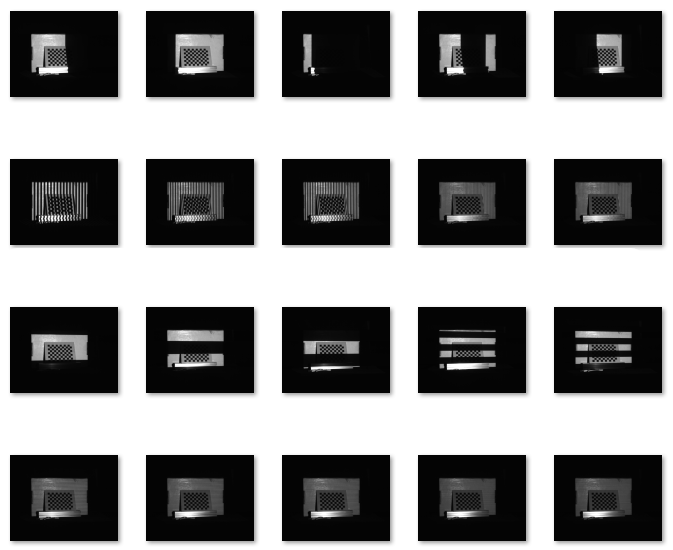
\includegraphics[scale=1]{9.png}
		\caption{标定过程拍摄的部分图像}
	\end{figure}

	而在三维重建模块,同样需要投影设计的编码结构光图案(如\ref{fig:fig1}所示),并对经过物体表面调制的图案进行拍摄。因此,在不同的两个模块均需要类 $Camera$ 和 $Projector$ 的实例,而由于在系统标定过程中,对相机的属性进行了改变,标定的结果与这些属性密切相关,如果在三维重建模块重新获得 $Camera$ 的实例进行拍摄,将导致物体三维坐标的计算产生一定的误差。此外,多次对 $Camera$ 和 $Projector$ 两个类进行实例化,也有可能导致异常的发生和资源的浪费。
	
	综上所述,本项目对类 $Camera$ 和 $Projector$ 采用了单例模式,保证相机和投影仪对应的类只有一个对应的实例被创建。
	
	本项目的类图如图\ref{fig:fig5}所示:
		\begin{figure}[!htbp]
		\centering
		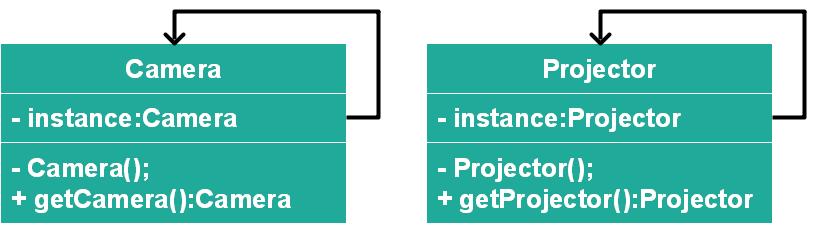
\includegraphics[scale=0.7]{13.png}
		\caption{项目类图}
		\label{fig:fig5}
	\end{figure}
	
	使用单例模式的优劣分别如下:
	\begin{itemize}
		\item \textbf{优势}
		\begin{itemize}
			\item[$\blacksquare$] 参与单例模式的类只有一个实例,对单例类的所有实例化得到的都是相同的一个实例。这样就防止其它对象对自己的实例化,确保所有的对象都访问一个实例 
			\item[$\blacksquare$] 单例模式具有一定的伸缩性,类自己来控制实例化进程,类就在改变实例化进程上有相应的伸缩性
			\item[$\blacksquare$] 提供了对唯一实例的受控访问
			\item[$\blacksquare$] 由于在系统内存中只存在一个对象,因此可以 节约系统资源,当需要频繁创建和销毁的对象时单例模式无疑可以提高系统的性能
			\item[$\blacksquare$] 避免对共享资源的多重占用。 
		\end{itemize}
			\item \textbf{劣势}
	\begin{itemize}
		\item[$\blacksquare$] 单例类的职责过重,在一定程度上违背了“单一职责原则”
		\item[$\blacksquare$] 滥用单例将带来一些负面问题,如实例化的对象长时间不被利用,系统会认为是垃圾而被回收,这将导致对象状态的丢失
		\item[$\blacksquare$] 由于单利模式中没有抽象层,因此单例类的扩展有很大的困难
	\end{itemize}
	\end{itemize}
\subsection{适配器模式}
适配器模式是一种结构型模式,可以使一个类和接口不匹配的其它类进行交互。适配器将一个类的接口转换为 $Client$ 类期望的另一个接口,让类可以协同工作,否则会因为接口不兼容而无法进行。

适配器模式的参与者包括:
\begin{itemize}
	\item $Target$:定义 $Client$ 使用的特定于某个域的接口
	\item $Adapter$:将 $Adaptee$ 接口适配到 $get$ 接口
	\item $Adoptee$:定义需要被适配的已有接口
	\item $Client$:与遵循 $Target$ 接口的对象协作
\end{itemize}

适配器可以分为两种:
\begin{enumerate}
	\item[(1)] \textbf{类适配器:}通过继承实现,从不兼容的类派生出新类并添加我们需要的方法使得派生类满足预期接口
	\item[(2)] \textbf{对象适配器:}通过对象组合实现,新类中包含原始类并且在新类里创建方法以实现调用的转换
\end{enumerate}

其类图如图\ref{fig:fig2}和图\ref{fig:fig3}所示:

	 	\begin{figure}[!htbp]
	\centering
	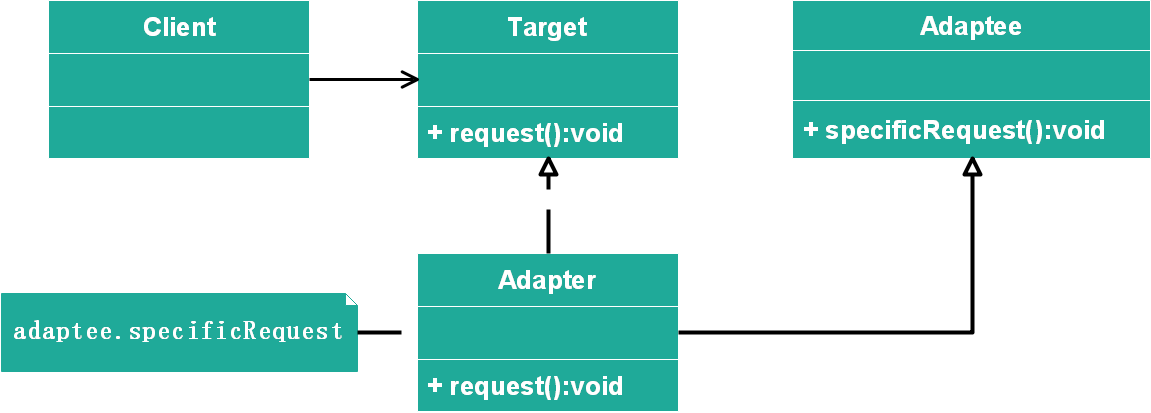
\includegraphics[scale=0.5]{10.png}
	\caption{适配器模式类图-类适配器}
	\label{fig:fig2}
\end{figure}

	 	\begin{figure}[!htbp]
	\centering
	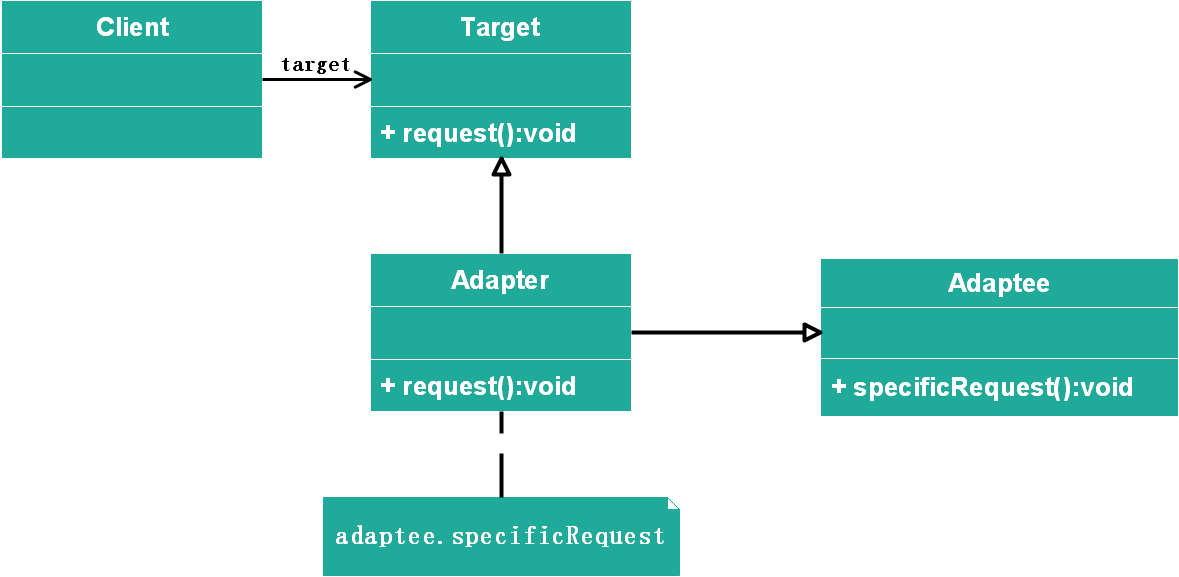
\includegraphics[scale=0.5]{11.png}
	\caption{适配器模式类图-对象适配器}
	\label{fig:fig3}
\end{figure}



本项目的用户界面基于 Qt \footnote{Qt 是一个跨平台的 C++ 应用程序开发框架,广泛用于开发 GUI 程序。}开发,相机拍摄的图像将展示在 Qt 开发的用户界面。类 $Camera$ 定义了内部类 $CameraFrame$,包含图像的分辨率(宽度和高度),图像内容和图像信息等,为了将相机视野展示在用户界面上,需要将自定义的 $CameraFrame$ 类转换为 Qt 的图片类 $QImage$。此外,在结构光解码过程中,依赖于 OpenCV\footnote{OpenCV 是一个跨平台的计算机视觉库,可用于开发实时的图像处理、计算机视觉以及模式识别程序。} 对图像进行处理,因此,在对图像进行结构光解码之前,也需要对接口进行转换。

本项目主要采用对象适配器,即通过对象组合实现。通过定义新的类 $CVTools$,在新类中包含 $CameraFrame$,$Mat$ 等类的对象,实现不同类型数据对象之间的转换,并定义新的方法提供 $Client$ 类可以调用的转换接口。

下面为将 $CameraFrame$ 转换为 OpenCV 中 $Mat$ 的适配器。
	 	\begin{figure}[!htbp]
	\centering
	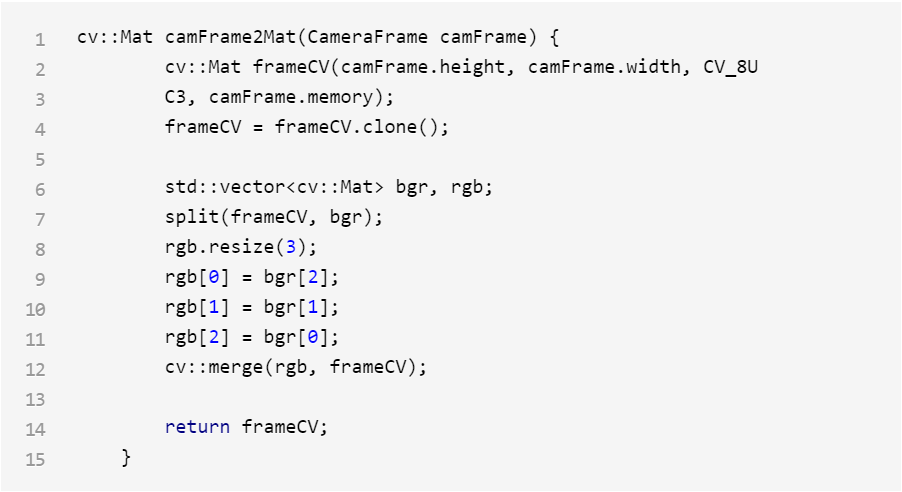
\includegraphics[scale=0.8]{12.png}
	\caption{CameraFrame-Mat Adapter}
\end{figure}

其类图如图\ref{fig:fig4}所示:
	 	\begin{figure}[!htbp]
	\centering
	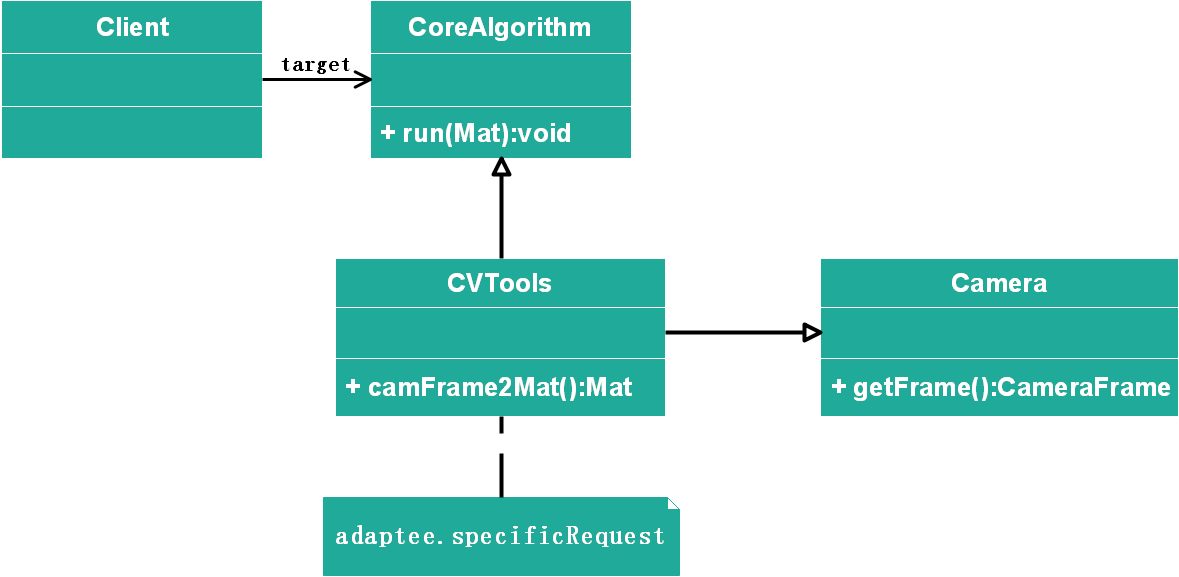
\includegraphics[scale=0.5]{14.png}
	\caption{CameraFrame-Mat Adapter}
	\label{fig:fig4}
\end{figure}

其中,$Camera$ 类为相机类,$getFrame()$ 方法控制相机拍摄并获得 $CameraFrame$ 对象,$CoreAlgorithm$ 类为进行结构光解码的类,是 $Client$ 类使用的特定接口,该接口需要 $Mat$ 对象作为输入参数,因此, $CVTools$ 类作为适配器对他们进行匹配,使得其可以协同工作。

使用对象适配器的优势在于一个对象适配器可以把多个不同的适配者适配到同一个目标。
可以适配一个适配者的子类,由于适配器和适配者之间是关联关系,根据“里氏替换原则”,适配者的子类也可通过该适配器进行适配。但与类适配器模式相比,要在适配器中置换适配者类的某些方法比较麻烦。如果一定要置换掉适配者类的一个或多个方法,可以先做一个适配者类的子类,将适配者类的方法置换掉,然后再把适配者类的子类当做真正的适配者进行适配,实现过程较为复杂。

\subsection{工厂模式}
工厂模式是一种创建者模式的设计模式,有工厂方法和抽象工厂两种变种。工厂模式的目的在于创建对象的过程中没有暴露对象的初始化逻辑给用户,仅通过一个公共接口引用最新创建的对象。

工厂模式适用于当类不能预测要创建哪个类的对象或当类引用其子类去定义要创建的对象的类型以及当对象的创建要局部化三种情形。

工厂模式的参与者包括:

\begin{itemize}
	\item Product:定义工厂方法要创建的对象的接口
	\item Concrete Product:实现 Product 接口
	\item Creator:声明工厂方法,返回一个产品类型的对象构造器也可能定义一种缺省的工厂方法,返回一个缺省的 Concrete Product对象
	\item Concrete Creator:	重写工厂方法来获得一个 Concrete Product的实例
\end{itemize}

其类图如下图所示:

	 	\begin{figure}[!htbp]
	\centering
	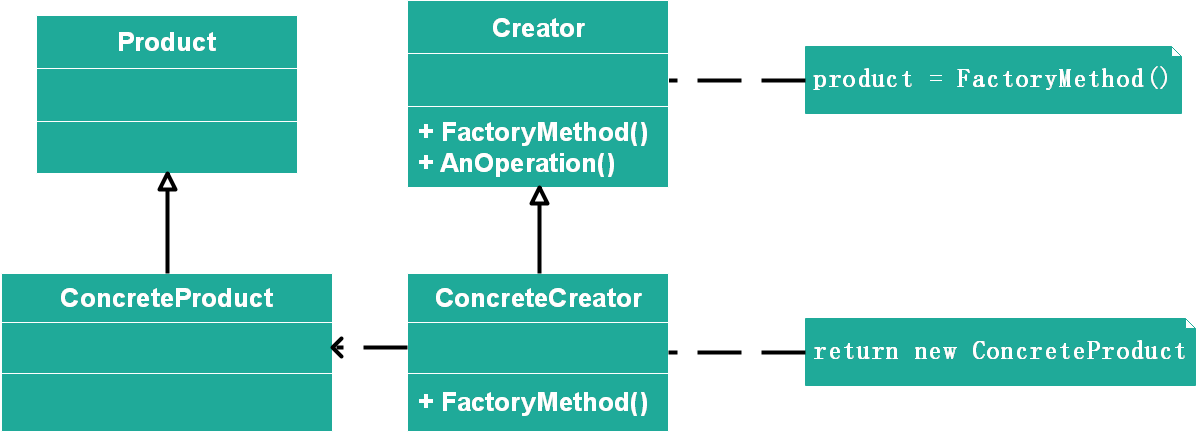
\includegraphics[scale=0.5]{15.png}
	\caption{工厂方法类图}
\end{figure}

点云是在三维重建后获得的物体表面海量点集合,包含点的三维坐标(XYZ)和颜色信息(RGB)。本系统的点云渲染模块主要是对点云的可视化和对用户事件的相应。该模块的开发依赖于PCL\footnote{PCL 是C ++编写的一个开源的点云算法库,支持点云的处理,可用于特征估计,表面重建,模型拟合和分割等}。PCL 中提供的点云对象包括 $PointXYZ$, $PointXYZRGB$, $PointXYZRGBA$, $PointXYZHSV$ 等,目前,项目对点云对象的处理为默认 $PointXYZRGB$ 并提供缺省颜色。其类图如图\ref{fig:fig6}所示。

\begin{figure}[!htbp]
	\centering
	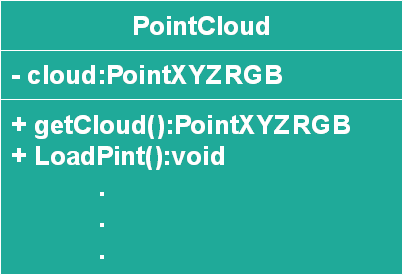
\includegraphics[scale=0.5]{16.png}
	\caption{项目原始类图}
	\label{fig:fig6}
\end{figure}

而通过工厂方法,在载入点云时,可根据点云文件(如$pcd$文件\footnote{PCD全称Point Cloud Data,是一种存储点云数据的文件格式,文件格式头(file format header)说明文件中存储的点云数据的格式。})的头部判断不同的点云对象,从而返回不同类型的点云对象。

修改后的类图如图\ref{fig:fig7}所示:

\begin{figure}[!htbp]
	\centering
	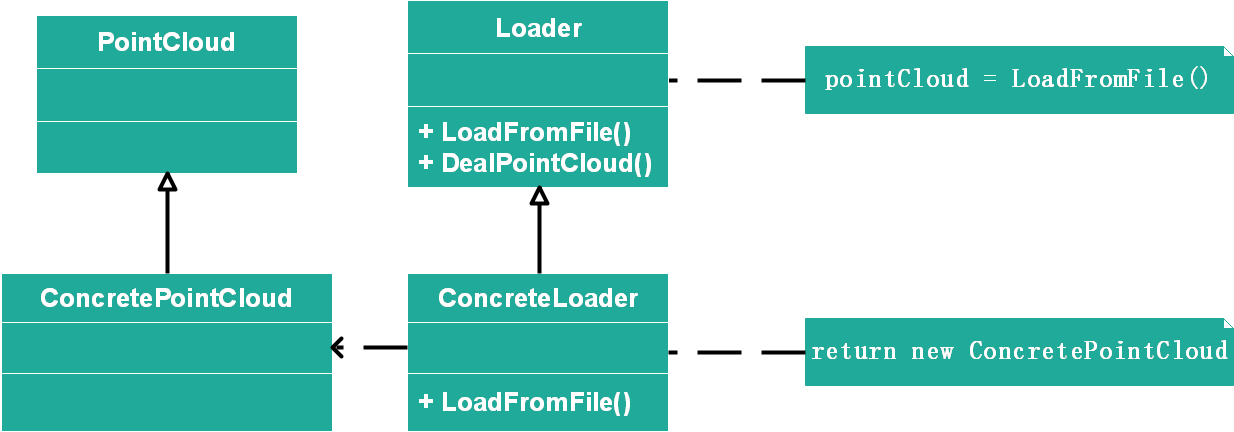
\includegraphics[scale=0.5]{17.png}
	\caption{项目修改类图}
		\label{fig:fig7}
\end{figure}

其中,$PointCloud$ 是点云对象的接口,定义了修改点云颜色、剔除异常点等方法,$ConcretePointCloud$ 实现了 $PointCloud$ 接口,有不同类型的点云对象。$Loader$ 声明了工厂方法,即从文件中读入点云的方法,$ConcreteLoader$ 重写工厂方法,根据文件中头部声明的不同点云类型来获得不同的 $ConcretePointCloud$ 的实例。

在工厂模式下,用户只需要关心所需产品对应的工厂,无须关心创建细节,甚至无须知道具体产品类的类名。使用工厂方法模式的另一个优点是在系统中加入新产品时,无须修改抽象工厂和抽象产品提供的接口,无须修改客户端,也无须修改其他的具体工厂和具体产品,而只要添加一个具体工厂和具体产品就可以了。这样,系统的可扩展性也就变得非常好,完全符合“开闭原则”。但在添加新产品时,需要编写新的具体产品类,而且还要提供与之对应的具体工厂类,系统中类的个数将成对增加,在一定程度上增加了系统的复杂度,有更多的类需要编译和运行,会给系统带来一些额外的开销。
	
\subsection{代理模式}

代理模式采用代理对象可以给用户提供更好的用户体验(也可以对目标对象的访问进行一定的控制)。例如,当页面还没加载过来的时候,代理对象可以提供一个状态条来显示,页面、图像加载到什么程度。

代理模式适用于当需要用简单对象表示复杂对象,或如果一个对象,譬如大的图像,需要很长时间来加载,尤其对象需要通过网络加载,网络负载高时可能很缓慢以及如果对象具有有限访问权限,则代理可以验证该用户的访问权限。

代理模式的参与对象包括:
\begin{itemize}
	\item Subject:由RealSubject实现的接口并代表其服务
	\item Proxy:维护Proxy访问RealSubject的引用,实现RealSubject实现的相同接口,以便Proxy替代RealSubject,	控制对RealSubject的访问,并可能负责其创建和删除,依赖于代理种类的其他职责
	\item RealSubject:Proxy代表的真实对象
	\end{itemize}
其类图如图\ref{fig:fig8}所示:
\begin{figure}[!htbp]
	\centering
	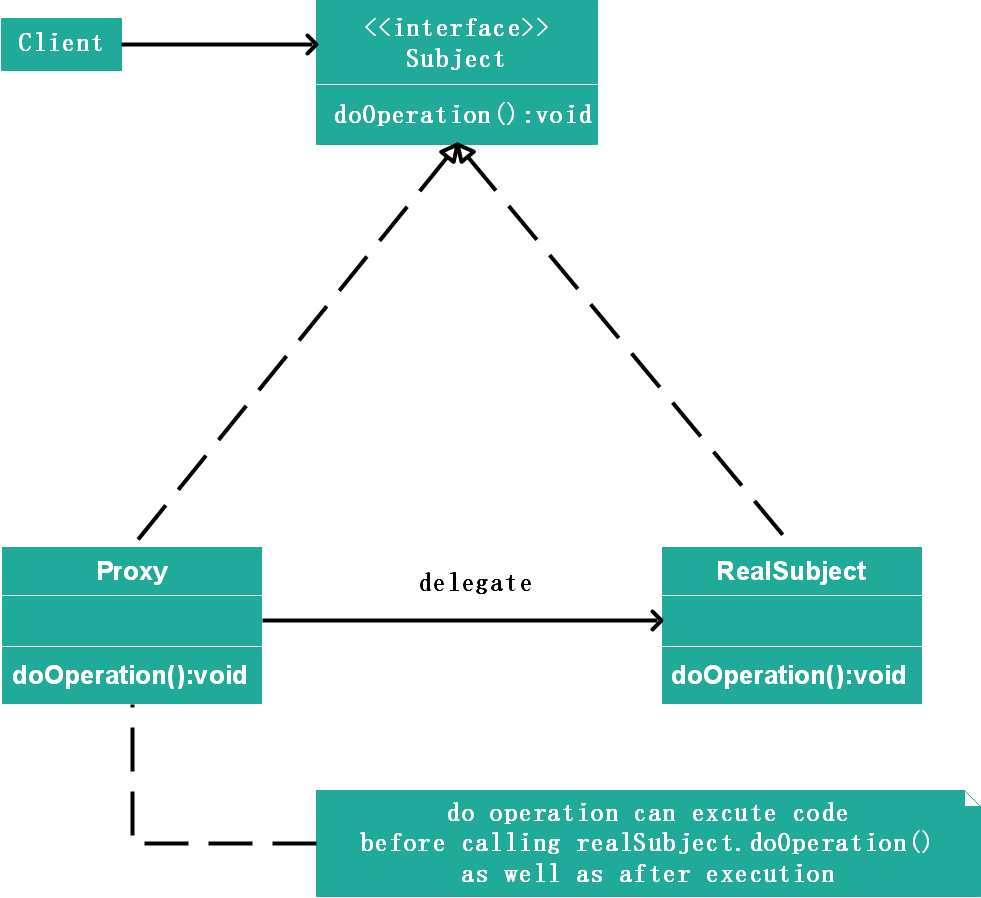
\includegraphics[scale=0.5]{18.png}
	\caption{代理模式类图}
	\label{fig:fig8}
\end{figure}

根据第二节的描述,本系统旨在对轮轨表面进行稠密重建,项目进行到现在,已经实现了在半径 95 mm 的球体单表面提取 17 W+ 的点云数据。在三维重建进行坐标计算的过程中或在将这些点云数据导入软件的过程中,由于数据量大而容易造成界面假死。

而项目使用代理模式即可解决这一问题。由于数据体量大,加载时间过长,可以在加载的时候辟一个线程,在新的线程中加载,加载完成后通过delegate协议将点云对象传给界面。在加载的过程中,可以通过进度条或加载界面等方式提示用户加载进度等。

项目的类图如图\ref{fig:fig9}所示:

\begin{figure}[!htbp]
	\centering
	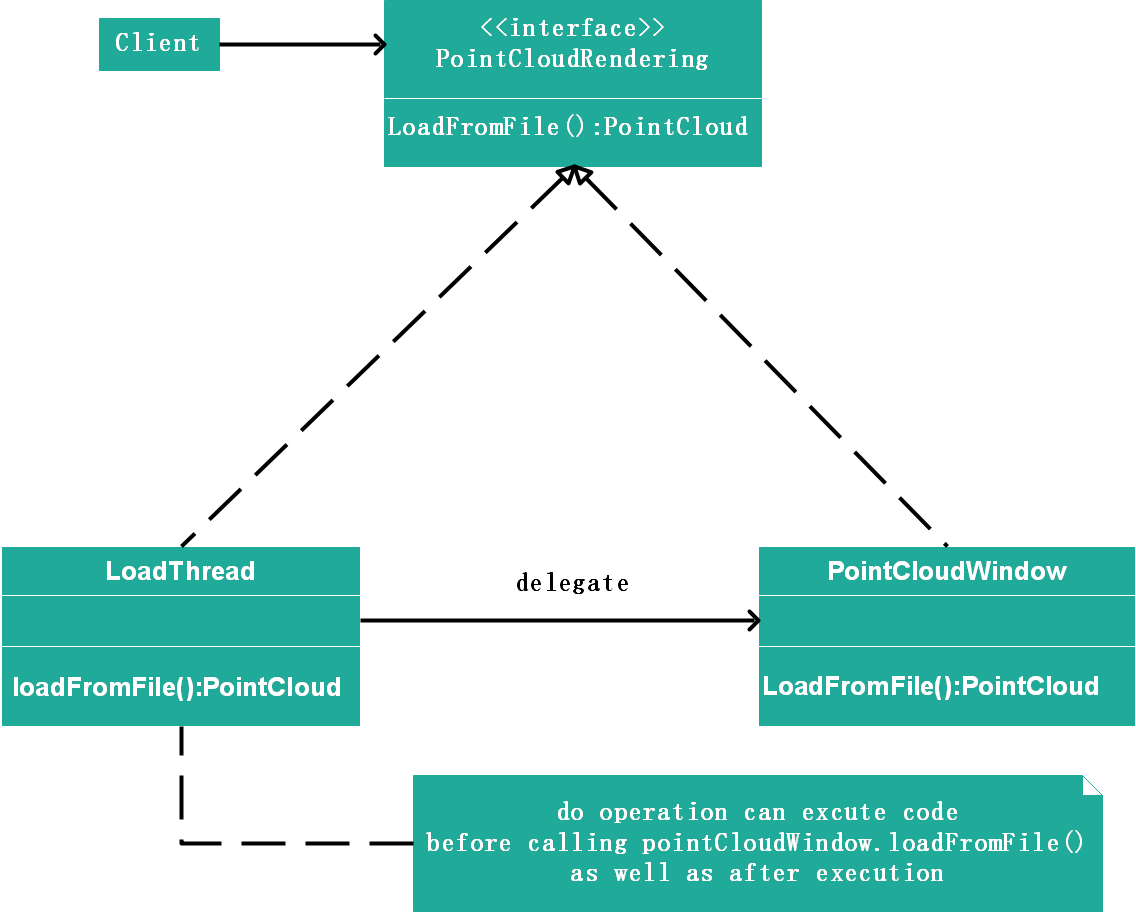
\includegraphics[scale=0.5]{19.png}
	\caption{项目类图}
	\label{fig:fig9}
\end{figure}

使用代理模式可以协调调用者和被调用者,在一定程度上降低了系统的耦合度。远程代理使得客户端可以访问在远程机器上的对象,远程机器可能具有更好的计算性能与处理速度,可以快速响应并处理客户端请求。虚拟代理通过使用一个小对象来代表一个大对象,可以减少系 统资源的消耗,对系统进行优化并提高运行速度。保护代理可以控制对真实对象的使用权限。但由于在客户端和真实主题之间增加了代理对象,因此 有些类型的代理模式可能会造成请求的处理速度变慢。而且实现代理模式需要额外的工作,有些代理模式的实现非常复杂。


\subsection{责任链模式}
	责任链模式通过为多个对象提供处理请求的机会,避免将请求的发送者耦合到其接受者。责任链模式将接收对象链接并沿链传递请求,直到对象处理它。链上的每个对象共享一个公共接口,用于处理请求和访问链上的后继者。
	
	责任链模式适用于当多个对象可以处理请求且事先不知道实际处理对象或当请求遵循“处理或转发”模型,也就说某些请求可在生成的地方处理,而其他请求必须转发到另一个对象处理以及希望能够动态修改可处理请求的对象集。此方法为在对象间分配职责提供了额外的灵活性。
	
	责任链模式的参与者包含:
	\begin{itemize}
		\item Handler:定义处理请求的接口,实现后继链接
	    \item  ConcreteHandler:处理他负责的请求,可以访问其继任者,如果 ConcreteHandler 可以处理请求,他会这样做,否则他会将请求转发给其继任者
		\item Client:启动对链上的 ConcreteHandler 对象的请求
	\end{itemize}
	
	其类图如图\ref{fig:fig10}所示:
	\begin{figure}[!htbp]
		\centering
		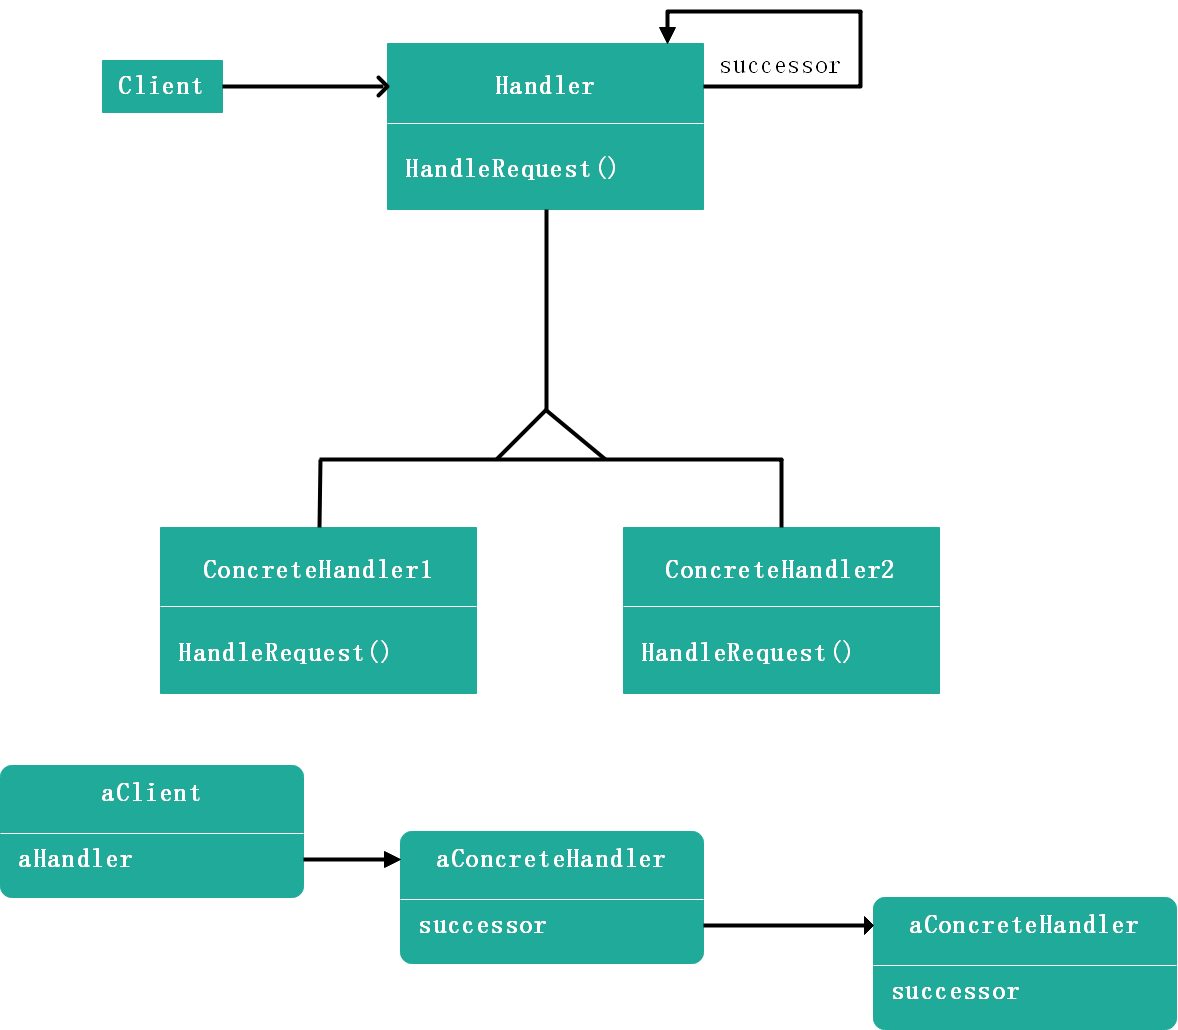
\includegraphics[scale=0.45]{20.png}
		\caption{责任链模式类图}
		\label{fig:fig10}
	\end{figure}
\newpage
	在本项目中,导入时读取的点云文件可能有多种文件类型,如 $pcd$, $ply$ 或 $txt$ 等。不同的文件格式需要调用不同的方法,现有项目通过判断文件类型来选择调用的方法,这样的设计不利于系统的扩展,当需要读取新的文件格式时,软件只能以修改源代码的方式满足需求,而不是以扩展的方式,违反了开放封闭原则。
	
		\begin{figure}[!htbp]
		\centering
		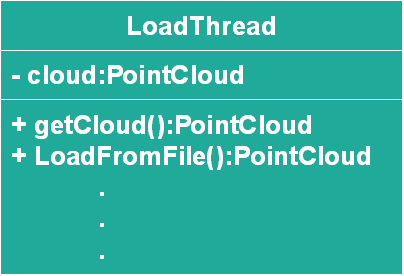
\includegraphics[scale=0.5]{21.png}
		\caption{项目原始类图}
	\end{figure}

	其中,方法 $LoadFromFile()$ 通过 $if-else$ 判断不同的文件类型,调用不同的方法。

	而进行重新设计使用责任链模式,链上的每个对象可以对文件类型进行判断,看是否可以进行处理,如果可以处理则将点云从文件中读入,否则将文件传给链上的后继。若最后没有对象可以处理该文件类型,则抛出警告或根据需要对软件进行扩展,添加新的对象处理该文件类型。
	
	修改后的项目类图如下图所示:
		\begin{figure}[!htbp]
		\centering
		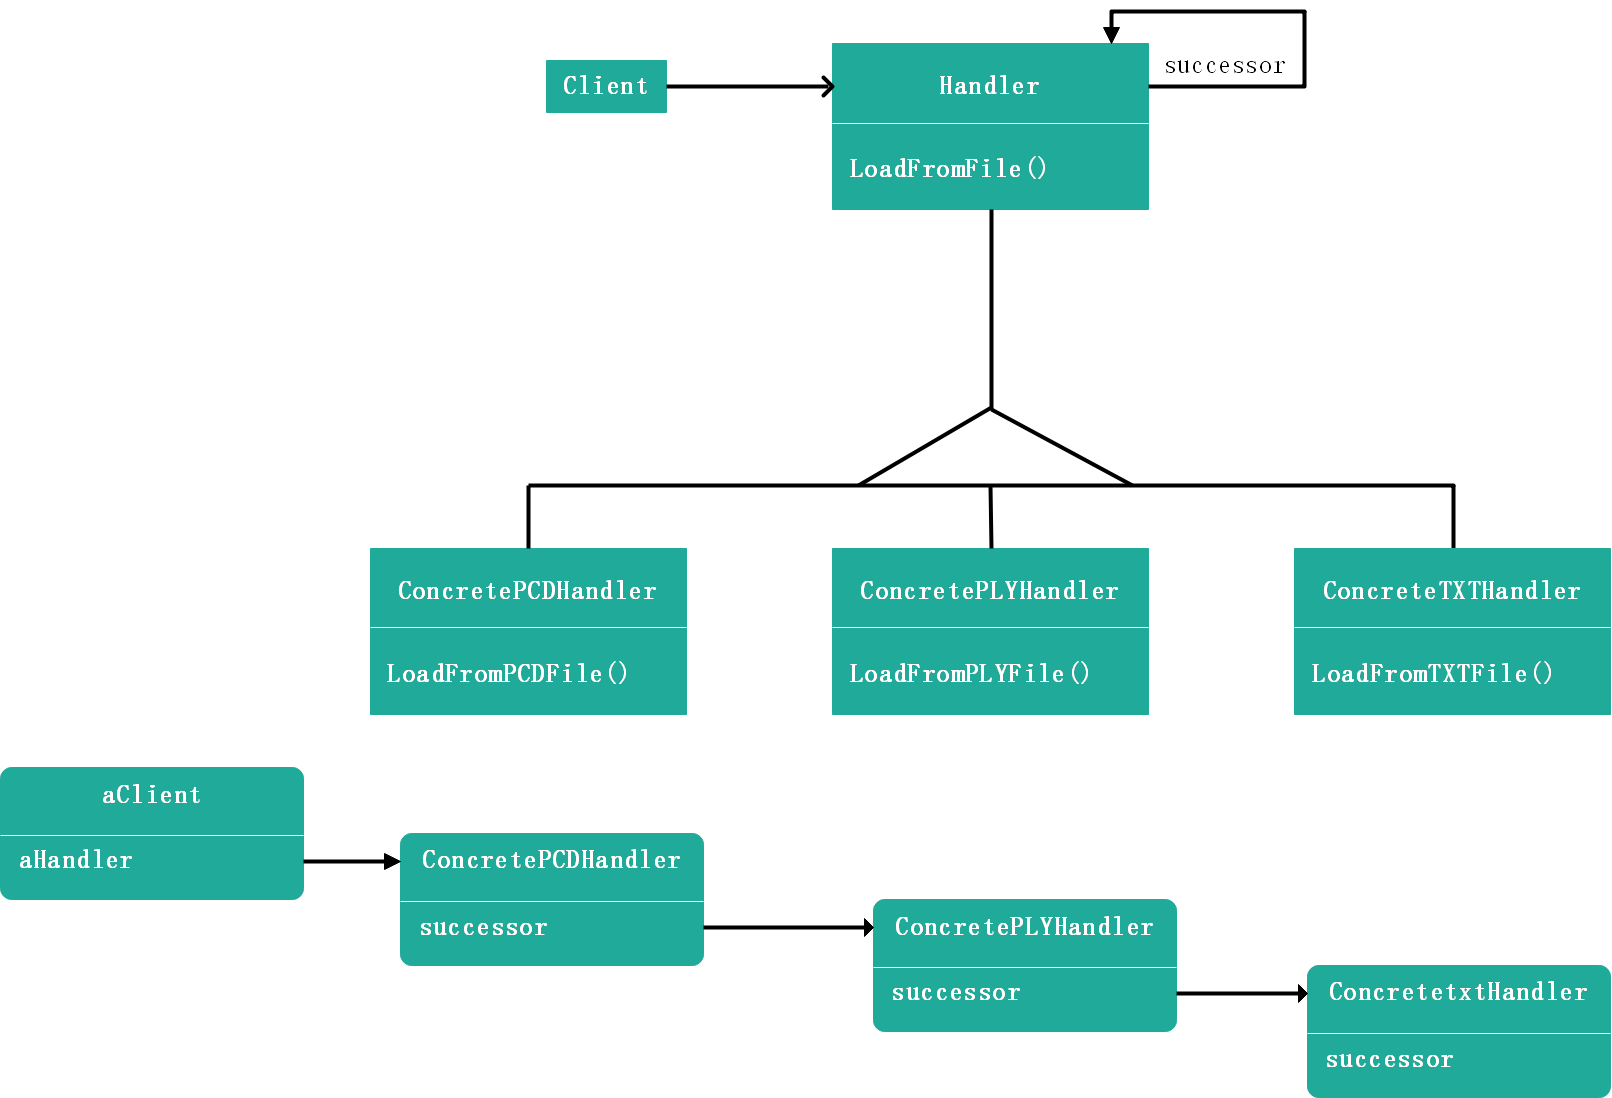
\includegraphics[scale=0.4]{22.png}
		\caption{项目修改类图}
	\end{figure}

	责任链模式有多种实现方法,本项目的实现拟采用在 Handler 接口中添加接收描述请求类型的修改方法,这种实现方法没有冗余且符合开放封闭原则。
	
	使用责任链模式的优点是链可以动态地修改,即可以根据需要动态地扩展软件处理文件的对象,缺点是必须分别在每个模块中实现链接,发送和转发代码。
	
	\section{项目总结}
	通过本文对结构光三维重建软件中已经运用的设计模式和可通过设计模式进行的改进分析,我们发现设计模式的运用可以解决软件设计和实现中存在的一些问题,通过这些可重用的解决方案优化软件的设计与实现。
	
	总体来说,设计模式的运用有以下几点好处:
	\begin{enumerate}
	\item[(1)] 复用解决方案——通过复用已经公认的设计,我能够在解决问题时取得先发优势,而且避免重蹈前人覆辙。我可以从学习他人的经验中获益,用不着为那些总是会重复出现的问题再次设计解决方案了。
	
	\item[(2)] 确立通用术语——开发中的交流和协作都需要共同的词汇基础和对问题的共识。设计模式在项目的分析和设计阶段提供了共同的基准点。
	
	\item[(3)] 提高观察高度--模式还为我们提供了观察问题、设计过程和面向对象的更高层次的视角,这将使我们从“过早处理细节”的桎梏中解放出来。
	
	\item[(4)] 大多数设计模式还能使软件更容易修改和维护。其原因在于,它们都是久经考验的解决方案。所以,它们的结构都是经过长期发展形成的,比新构思的解决方案更善于应对变化。而且,这些模式所用代码往往更易于理解——从而使代码更易维护。
	\end{enumerate}

	
	
	
\end{document}